%%%%%%%%%%%%%%%%%%%%%%%%%%%%%%%%%%%%%%%%%
% Beamer Presentation
% LaTeX Template
% Version 1.0 (10/11/12)
%
% This template has been downloaded from:
% http://www.LaTeXTemplates.com
%
% License:
% CC BY-NC-SA 3.0 (http://creativecommons.org/licenses/by-nc-sa/3.0/)
%
%%%%%%%%%%%%%%%%%%%%%%%%%%%%%%%%%%%%%%%%%

%----------------------------------------------------------------------------------------
%	PACKAGES AND THEMES
%----------------------------------------------------------------------------------------

\documentclass{beamer}

\mode<presentation> {

% The Beamer class comes with a number of default slide themes
% which change the colors and layouts of slides. Below this is a list
% of all the themes, uncomment each in turn to see what they look like.

%\usetheme{default}
%\usetheme{AnnArbor}
%\usetheme{Antibes}
%\usetheme{Bergen}
%\usetheme{Berkeley}
%\usetheme{Berlin}
%\usetheme{Boadilla}
\usetheme{CambridgeUS}
%\usetheme{Copenhagen}
%\usetheme{Darmstadt}
%\usetheme{Dresden}
%\usetheme{Frankfurt}
%\usetheme{Goettingen}
%\usetheme{Hannover}
%\usetheme{Ilmenau}
%\usetheme{JuanLesPins}
%\usetheme{Luebeck}
%\usetheme{Madrid}
%\usetheme{Malmoe}
%\usetheme{Marburg}
%\usetheme{Montpellier}
%\usetheme{PaloAlto}
%\usetheme{Pittsburgh}
%\usetheme{Rochester}
%\usetheme{Singapore}
%\usetheme{Szeged}
%\usetheme{Warsaw}

% As well as themes, the Beamer class has a number of color themes
% for any slide theme. Uncomment each of these in turn to see how it
% changes the colors of your current slide theme.

%\usecolortheme{albatross}
%\usecolortheme{beaver}
%\usecolortheme{beetle}
%\usecolortheme{crane}
%\usecolortheme{dolphin}
%\usecolortheme{dove}
%\usecolortheme{fly}
%\usecolortheme{lily}
%\usecolortheme{orchid}
%\usecolortheme{rose}
\usecolortheme{seagull}
%\usecolortheme{seahorse}
%\usecolortheme{whale}
%\usecolortheme{wolverine}

%\setbeamertemplate{footline} % To remove the footer line in all slides uncomment this line
%\setbeamertemplate{footline}[page number] % To replace the footer line in all slides with a simple slide count uncomment this line

%\setbeamertemplate{navigation symbols}{} % To remove the navigation symbols from the bottom of all slides uncomment this line
}



\newcommand\Fontv{\fontsize{5}{6.2}\selectfont}
\newcommand\Fontvi{\fontsize{6}{7.2}\selectfont}
\newcommand\Fontvii{\fontsize{7}{8.2}\selectfont}
\newcommand\Fontviii{\fontsize{8}{9.2}\selectfont}
\newcommand\Fontviiii{\fontsize{9}{10.2}\selectfont}

\setbeamerfont{caption}{series=\normalfont,size=\fontsize{6}{7.2}} 

\usepackage{graphicx} % Allows including images
\usepackage{booktabs} % Allows the use of \toprule, \midrule and \bottomrule in tables

%----------------------------------------------------------------------------------------
%	TITLE PAGE
%----------------------------------------------------------------------------------------

\title[Drawdown project]{Monthly Presentation of Drawdown project} % The short title appears at the bottom of every slide, the full title is only on the title page

\author{Boying Gong, Xinyue Zhou} % Your name
\institute[UC Berkeley] % Your institution as it will appear on the bottom of every slide, may be shorthand to save space
{
University of California, Berkeley \\ % Your institution for the title page
\medskip
\textit{jorothy\_gong@berkeley.edu \\}
\textit{xinyue233@berkeley.edu} % Your email address
}
\date{\today} % Date, can be changed to a custom date

\begin{document}

\begin{frame}
\titlepage % Print the title page as the first slide
\end{frame}

\begin{frame}
\frametitle{Overview} % Table of contents slide, comment this block out to remove it
\tableofcontents % Throughout your presentation, if you choose to use \section{} and \subsection{} commands, these will automatically be printed on this slide as an overview of your presentation
\end{frame}

%----------------------------------------------------------------------------------------
%	PRESENTATION SLIDES
%----------------------------------------------------------------------------------------

%------------------------------------------------
\section{Maximum drawdown distribution and CED}
%------------------------------------------------

\begin{frame}
\frametitle{Maximum drawdown distribution}
\Fontviii

As we move to longer period, the maximum drawdown distribution tends to:
\begin{enumerate}
\item have larger mean and variance
\item be multi-mode 
\item lack variability of values
\item be centered around several specific values
\end{enumerate}

Take RMZ as an example. (RMZ: The MSCI US REIT Index, a free float-adjusted market capitalization index that is comprised of equity REITs.)

\begin{figure}[h]
\Fontvii
\centering 
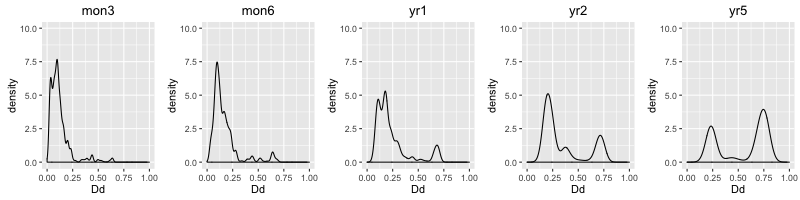
\includegraphics[width = 0.8\textwidth]{../results/maxdd_RMZ}
\caption{Maximum drawdown distribution of RMZ as rolling period increases} 
\label{fig: dmaxdd_RMZ}
\end{figure}

Later in our project, we mainly use 3 month period.

\end{frame}

%------------------------------------------------

\begin{frame}
\frametitle{High Correlation between Risk Measures}
\Fontviii

Maximum drawdown, expected shortfall (ES), value at risk (VaR) and volatility are highly correlated. For our 10 assets of interest, the correlation between the later three are all above 90\%. The correlation between maximum drawdown and the later three are weaker with an average around 80\%. \par
The following figure shows the rolling risk measures of RMZ.


\begin{figure}[h]
\centering 
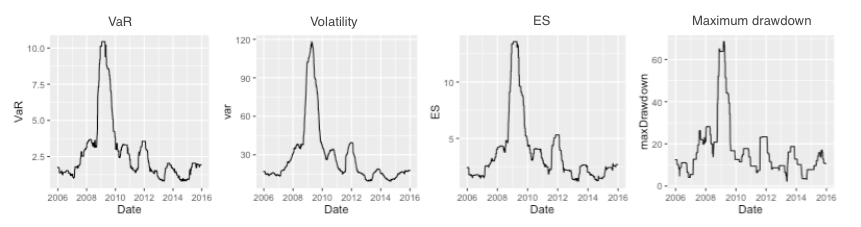
\includegraphics[width = 0.8\textwidth]{../results/risk_measure_RMZ}
\label{fig: risk_meausre_RMZ}
\caption{Comparison of different risk measures of RMZ} 
\end{figure}

\end{frame}

%------------------------------------------------

\begin{frame}
\frametitle{CED}
\Fontviii
\begin{columns}[c] % The "c" option specifies centered vertical alignment while the "t" option is used for top vertical alignment

\column{.35\textwidth} % Left column and width
The right column shows the rolling CED under 3-month-2-year Rolling Window (confidence level = 0.9). That means, the maximum drawdowns are calculated based on a 3-month rolling window and the tail means are calculated based on 2-year maximum drawdowns.

\column{.6\textwidth} % Right column and width
\begin{figure}[h]
\centering 
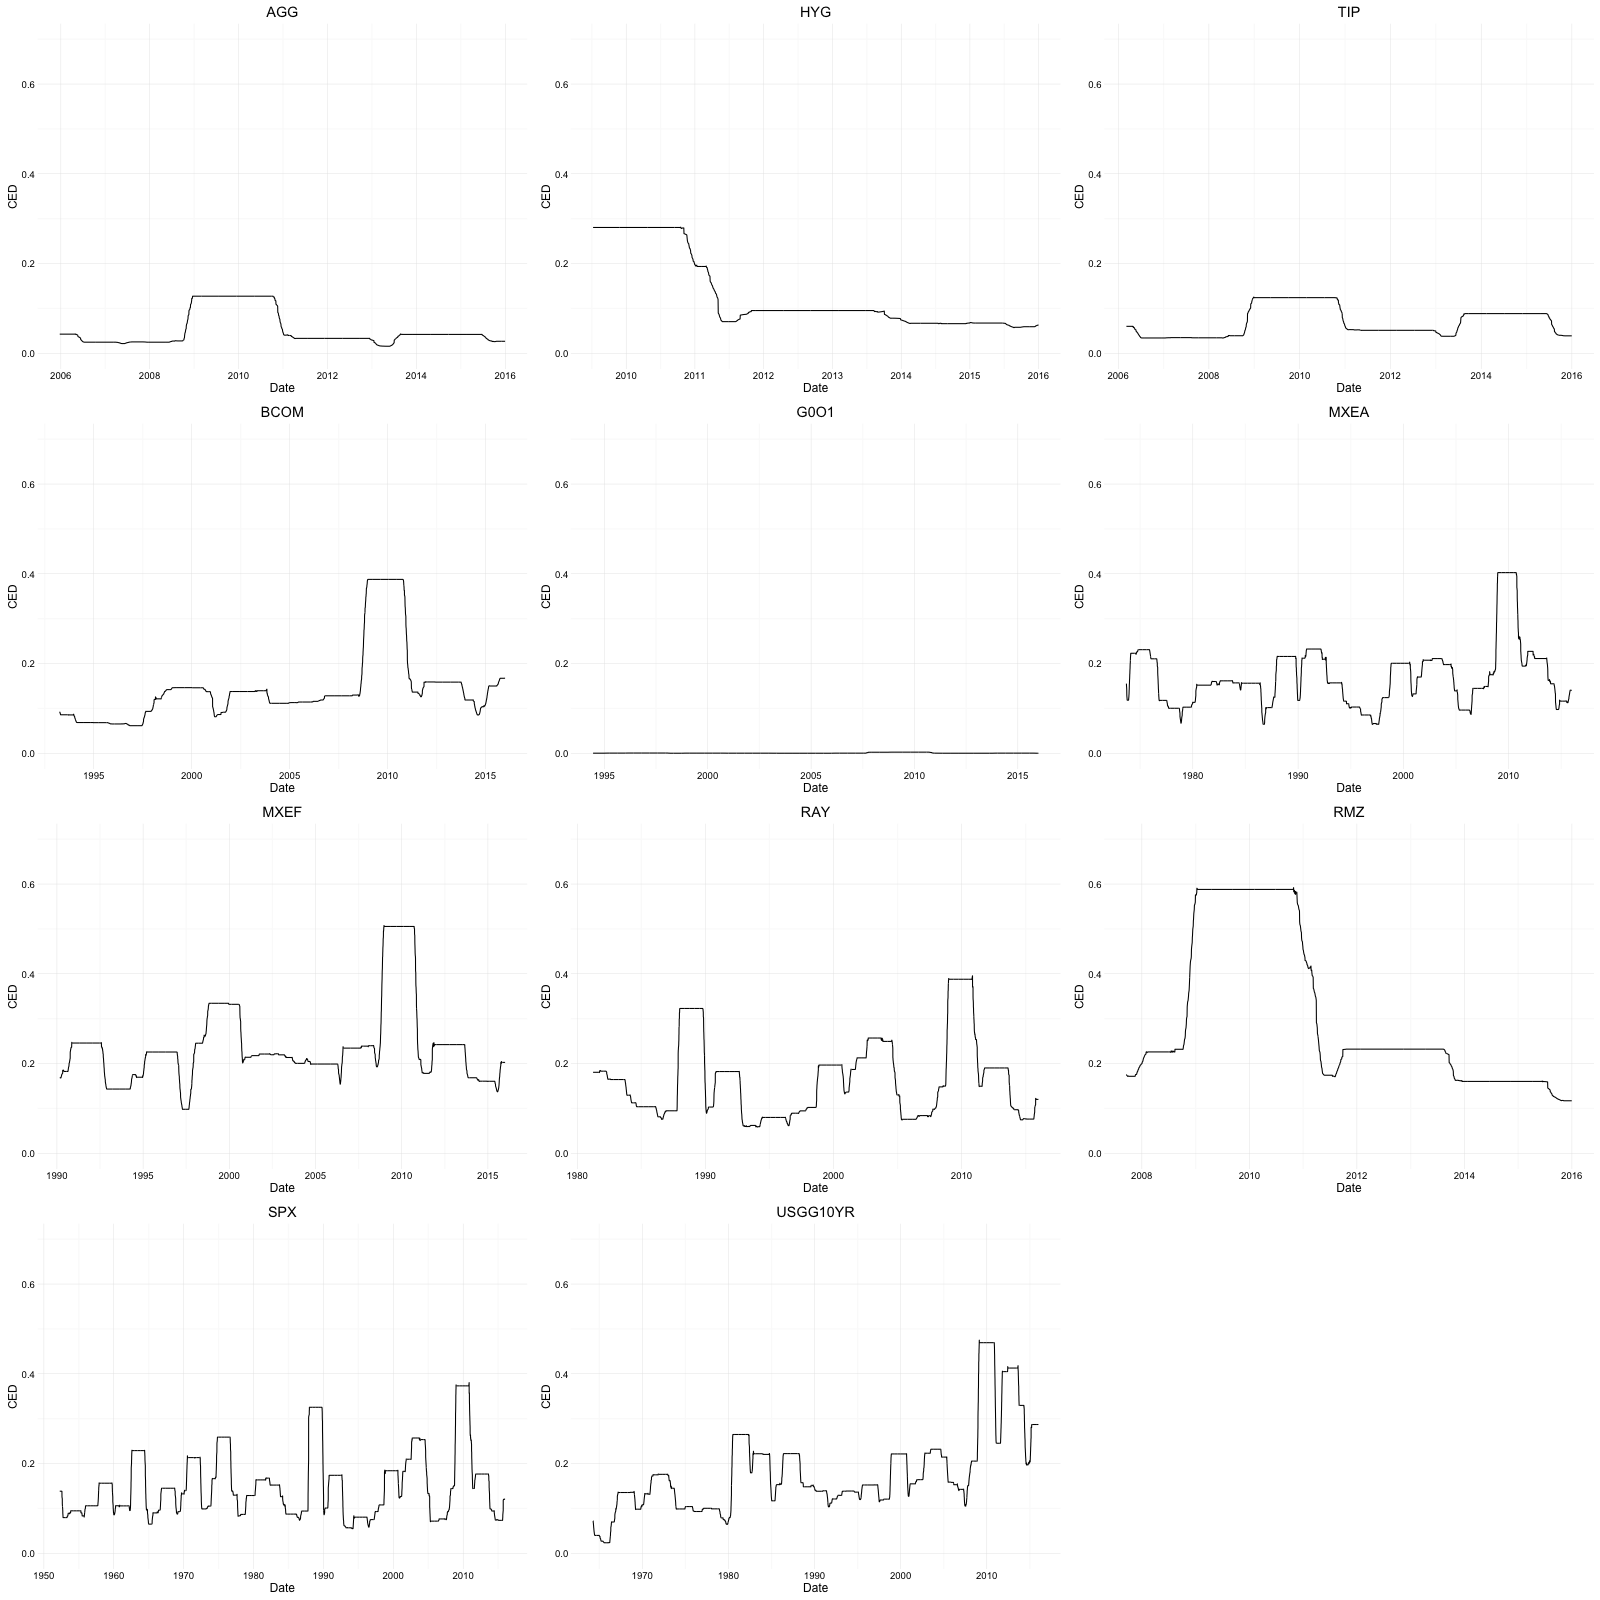
\includegraphics[width=1\textwidth]{../figures/rolling_stats/CED3mon2yr_scaled}
\label{fig: CED3mon2yr}
\end{figure}
\end{columns}
\end{frame}

%------------------------------------------------

\begin{frame}
\frametitle{CED}
\Fontviii

Note that CED is also highly correlated with other risk measures. The following table is calculated based on 2 year and 3 month rolling windows.

\begin{table}[!h]
\centering 
\begin{tabular}{ p{2cm}||p{2cm}|p{2cm}|p{2cm}} 
\hline
Measures & Volatility & VaR & ES\\
  \hline
AGG & 0.94 & 0.89 & 0.95\\ 
HYG & 0.98 & 0.97 & 0.97\\ 
TIP & 0.77 & 0.85 & 0.85\\ 
BCOM & 0.84 & 0.89 & 0.89\\ 
MXEA & 0.84 & 0.83 & 0.86\\ 
MXEF & 0.91 & 0.91 & 0.93\\ 
RAY & 0.92 & 0.85 & 0.92\\ 
RMZ & 0.96 & 0.96 & 0.97\\ 
SPX & 0.84 & 0.81 & 0.84\\ 
USGG10YR & 0.91 & 0.93 & 0.95\\
\hline
\end{tabular}
\label{table:corrRiskMeasureCED}
\caption{Correlation between CED (confidence level = 0.9) and other risk measures}
\end{table}

\end{frame}

%------------------------------------------------
\section{Time Series – ARMA model}
%------------------------------------------------

%------------------------------------------------
\subsection{Motivations}
\begin{frame}
\frametitle{Motivations}
\Fontviii
\begin{columns}[c]
\column{.35\textwidth} % Left column and width
\begin{enumerate}
\item Find a correct model to characterize the returns of financial assets. 
\item Check the relationship between serial correlations (here we use $\kappa(1)$) and risk measurements.
\end{enumerate}

\column{.6\textwidth} % Right column and width
\begin{figure}[h]
\centering 
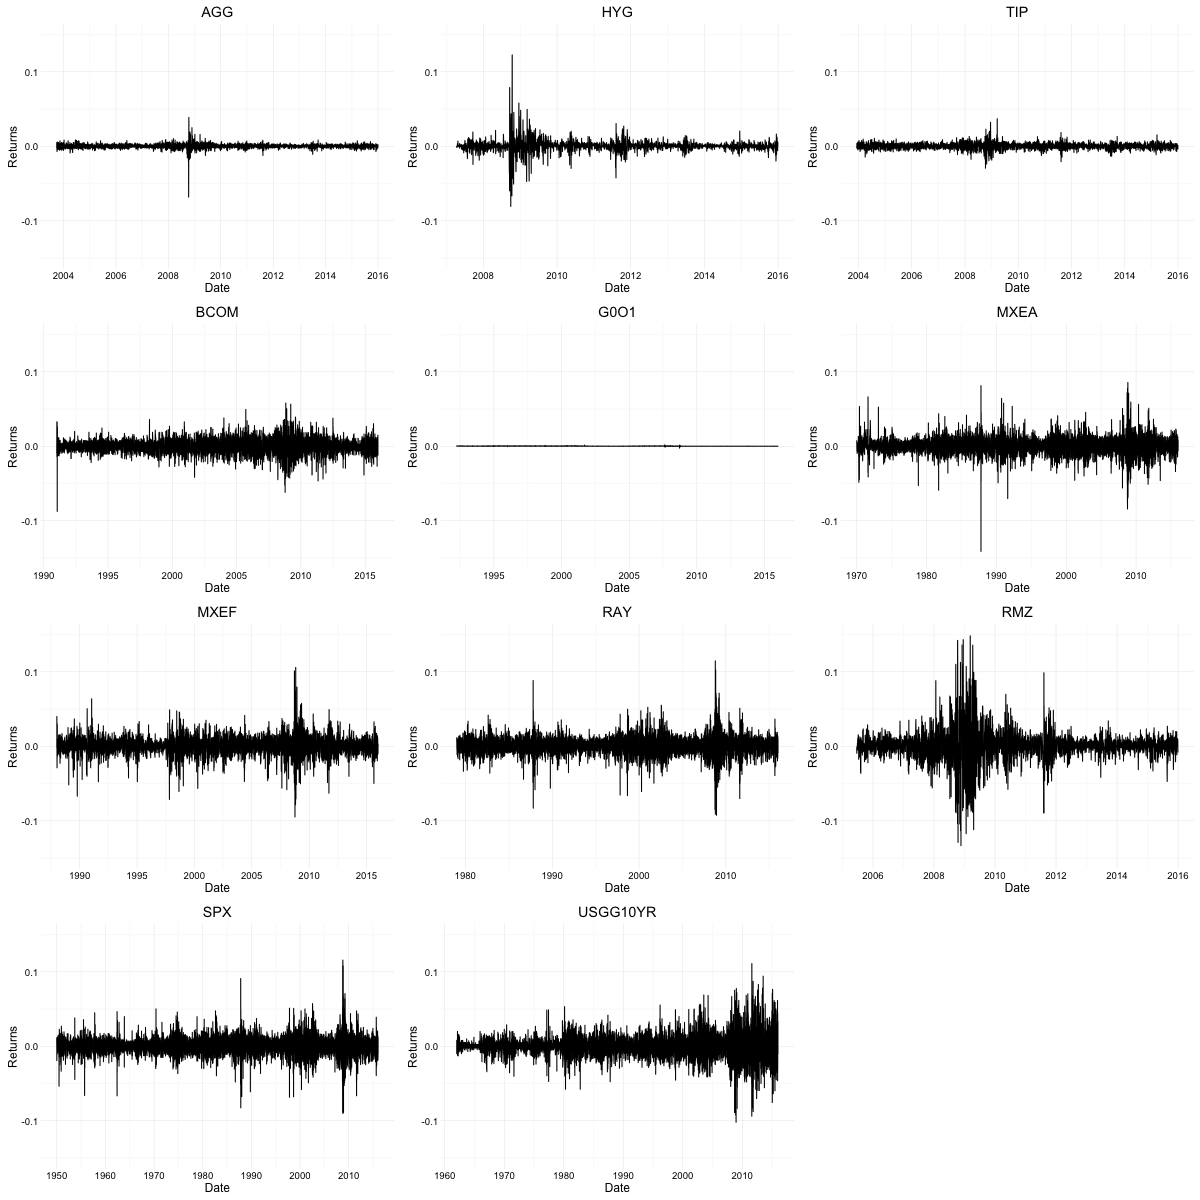
\includegraphics[width=6cm]{../figures/summary_daily/returns}
\label{fig: dailyReturns}
\caption{Daily Returns}
\end{figure}

\end{columns}
\end{frame}

\subsection{Serial Correlation and Risk Measurements under ARIMA Model}
\begin{frame}
\frametitle{$\kappa$(1) and Risk Measurements}
\Fontviii
\begin{columns}[c] % The "c" option specifies centered vertical alignment while the "t" option is used for top vertical alignment

\column{.35\textwidth} % Left column and width
\begin{enumerate}
\item Time series models
\begin{itemize}
\item AR(1)
\item MA(1)
\item ARMA(1,1)
\end{itemize}
\item Risk measurements
\begin{itemize}
\item VaR
\item ES
\item CED
\end{itemize}
\end{enumerate}

\column{.6\textwidth} % Right column and width
\begin{figure}[h]
\centering 
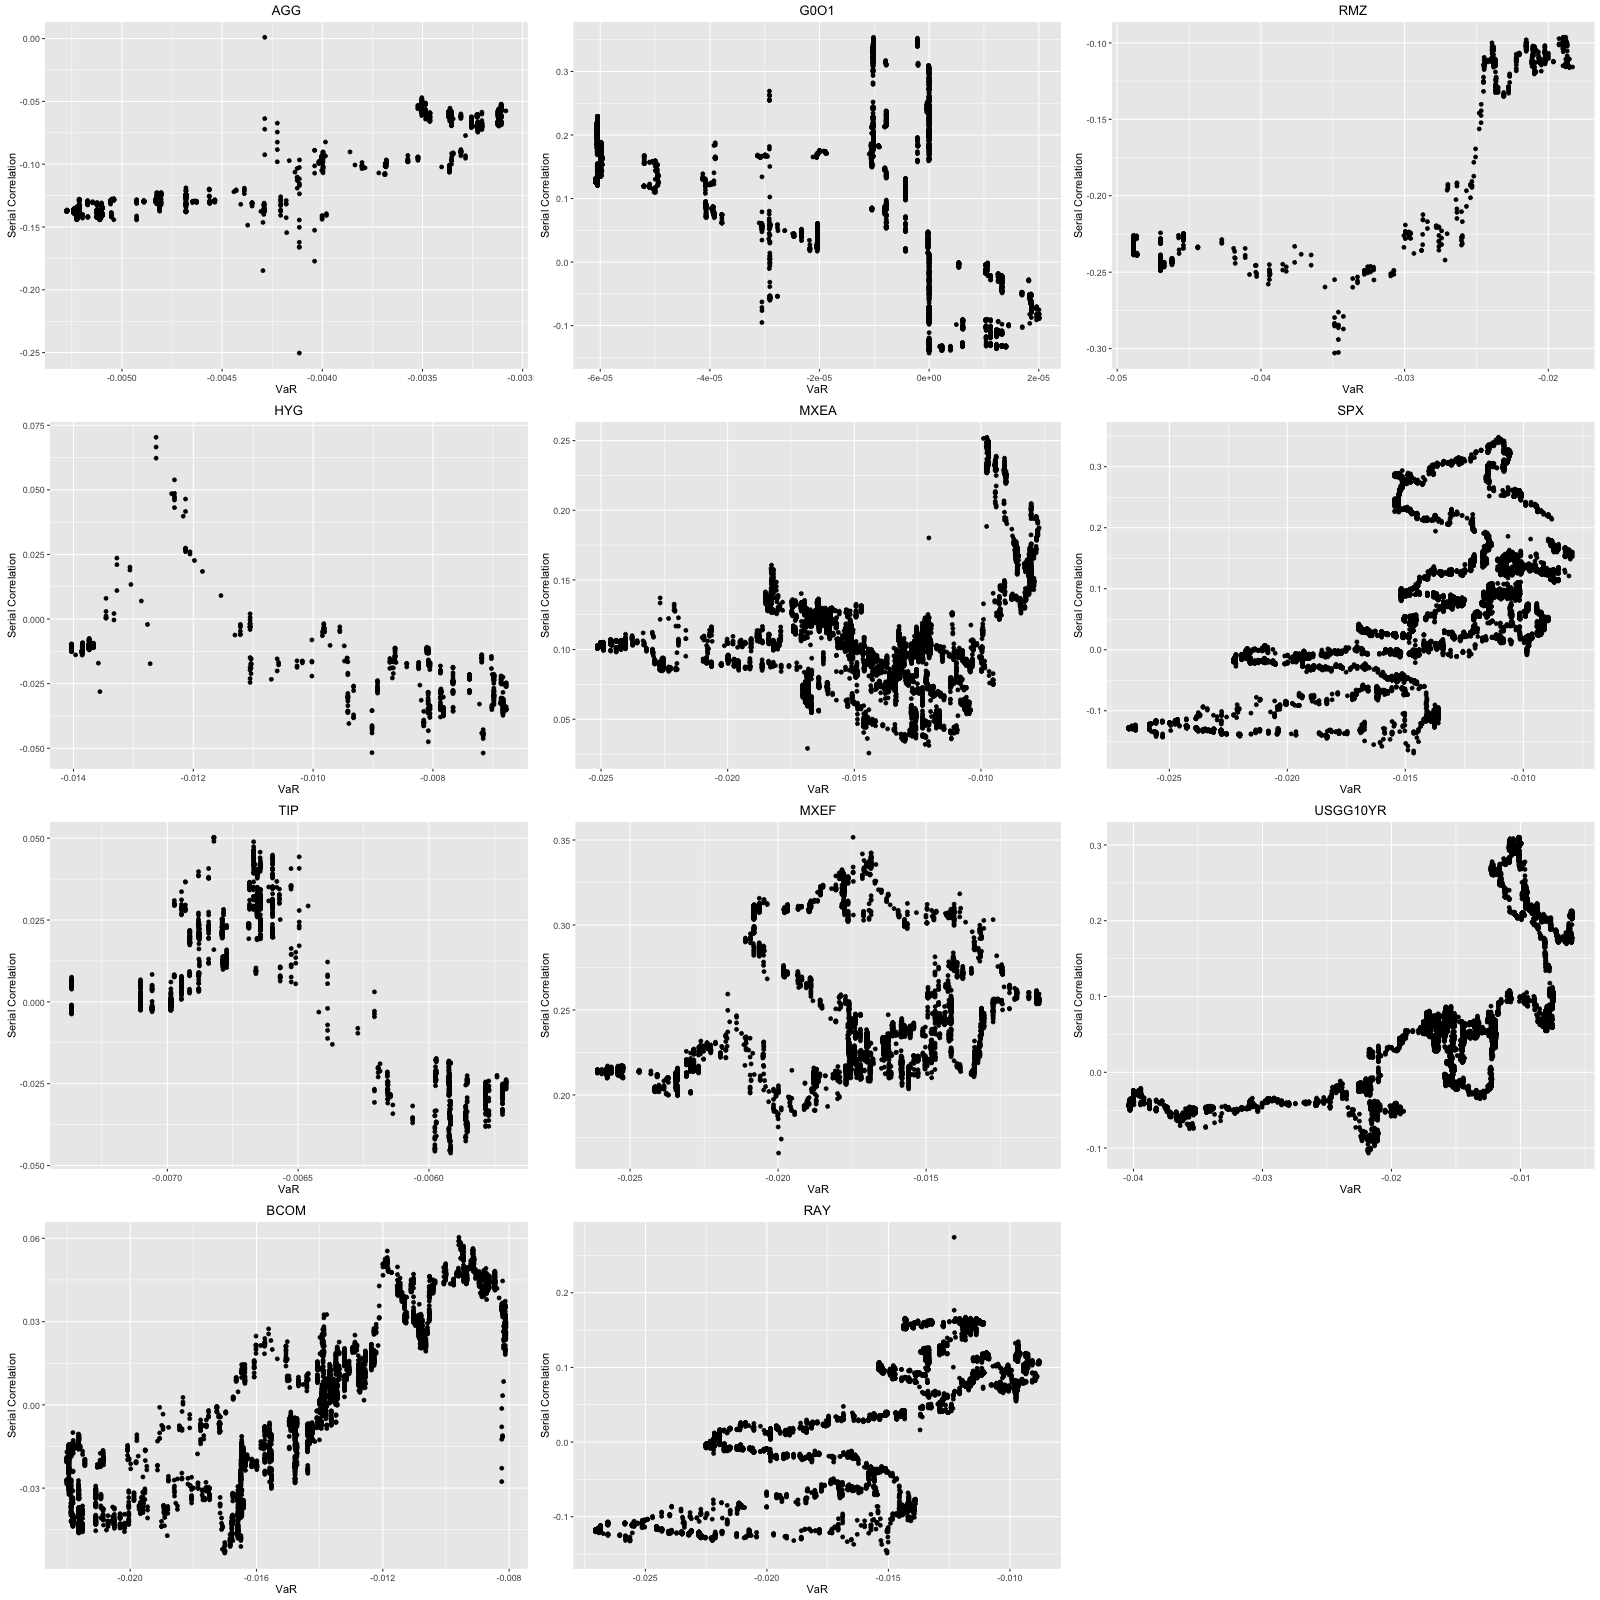
\includegraphics[width=6cm]{../results/SerCol-VaR5yrAR1}
\label{fig:SerCol-VaR5yrAR1}
\caption{AR(1): $\kappa(1)$ versus VaR}
\end{figure}
\end{columns}
\end{frame}


\subsection{Summary of ARMA}
\begin{frame}
\frametitle{ARMA is not enough...}
\Fontviii
\begin{columns}[c]
\column{.35\textwidth} % Left column and width
\begin{enumerate}
\item Inherently non-stationary
\item Clustered Variance
\begin{itemize}
\item Regime Model
\item GARCH Model
\end{itemize}
\end{enumerate}

\column{.6\textwidth} % Right column and width
\begin{figure}[h]
\centering 
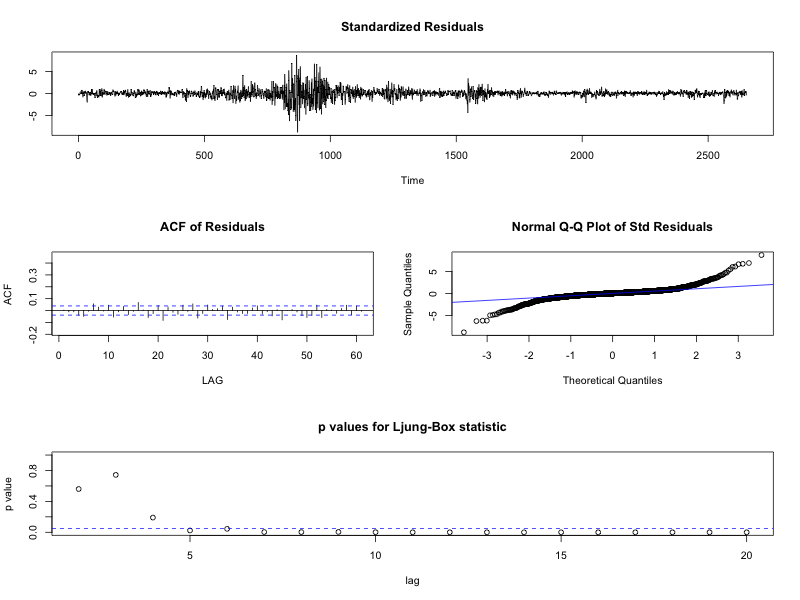
\includegraphics[width=6cm,height = 6cm]{../results/DiagnosticRMZ}
\label{fig: dailyReturns}
\caption{Fit RMZ Data using MA(1)}
\end{figure}

\end{columns}
\end{frame}

%------------------------------------------------
\section{Regime switching models}
%------------------------------------------------

\begin{frame}
\frametitle{Regime switching models}
\Fontviii
Many economic time series data tend to behave differently in adjacent time period. We use the following two-regime switching model to fit the returns:

\begin{equation}
y_t - \mu_{s^*_t} = \phi_{s^*_t} (y_{t-1} - \mu_{s^*_{t-1}}) + \epsilon_t
\end{equation}
where the number of autoregressive coefficient is set to 1. $s^*_t$ is a two state Markov chain. $s^*_t = 1$ represent regime 1 and $s^*_t = 2$ represent regime 2. $s^*_t$ depends on the past only through the most recent values:

\begin{equation}
P(s_t = j|s_{t-1}, s_{t-2}, \dots) = P(s_t = j|s_{t-1})  = p_{ij}
\end{equation}

\begin{table}[!h]
\centering 
\begin{tabular}{ | c || r  r | } 
 \hline
 & Regime 1  & Regime 2\\
Asset & High volatility  & Low volatility \\
  \hline \hline
AGG  & -0.134 & -0.114 \\ 
HYG & -0.010 &  0.025 \\ 
TIP &  0.039  & -0.026 \\ 
BCOM & -0.046 &  0.050 \\ 
MXEA & 0.095 & 0.109 \\ 
MXEF & 0.221 & 0.254 \\ 
RAY& -0.039  &  0.052 \\ 
RMZ & -0.244 &  0.007 \\ 
SPX & -0.018 &  0.113 \\ 
USGG10YR & -0.031 & 0.082 \\ 
 \hline
\end{tabular}
\label{table:autoCoeffRegime}
\caption{$\phi$ of high and low volatility regimes for various assets} 
\end{table}
\end{frame}

%------------------------------------------------

\begin{frame}
\frametitle{Regime switching models}
\Fontviii

Returns of high volatility regime has larger standard deviation, skewness and kurtosis than that of the low volatility regime. The return distribution of high volatility regimes are more like to be sknewed (both positive and negative). They also tend to have fatter tailed than the return distribution of low volatility regimes.

\begin{table}[!h]
\centering 
\begin{tabular}{ | c || rr | rr | rr | } 
 \hline
& \multicolumn{2}{c|}{Volatility} & \multicolumn{2}{c|}{Skewness} & \multicolumn{2}{c|}{Kurtosis} \\
Asset & Regime 1 & Regime 2 & Regime 1 & Regime 2 & Regime 1 & Regime 2 \\
  \hline \hline
AGG & 0.141 & 0.036 & -1.59 &  0.01 & 17.15 &  0.60\\ 
HYG & 0.265 & 0.055 &  0.60 &  0.00 &  8.76 &  0.83\\ 
TIP & 0.113 & 0.049 &  0.18 & -0.06 &  2.50 &  0.16\\ 
BCOM & 0.205 & 0.096 & -0.25 & -0.04 &  1.92 &  0.28\\ 
MXEA & 0.253 & 0.101 & -0.14 & -0.02 &  4.26 &  0.25\\ 
MXEF & 0.303 & 0.119 & -0.08 & -0.06 &  2.39 &  0.38\\ 
RAY & 0.307 & 0.114 & -0.39 & -0.06 &  6.43 &  0.55\\ 
RMZ & 0.661 & 0.159 &  0.29 & -0.15 &  2.92 &  0.79\\ 
SPX & 0.260 & 0.099 & -0.43 & -0.02 &  9.11 &  0.56\\ 
USGG10YR & 0.314 & 0.098 &  0.09 & -0.05 &  2.67 &  1.17 \\
 \hline
\end{tabular}
\label{table:statSumRegime}
\caption{Summary statistics of two regimes for various assets} 
\end{table}
\end{frame}

%------------------------------------------------

\begin{frame}
\frametitle{Regime switching models--Example: RMZ}
\Fontviii

\begin{columns}[c] % The "c" option specifies centered vertical alignment while the "t" option is used for top vertical alignment

\column{.4\textwidth} % Left column and width
The right panel shows the regime plot of RMZ returns and its smoothed probabilities. The regime switching model seperate the 2008 financial crisis as high volatilty regimes. The number of trading days of high and low volatility regime is 699 and 1954 seperately.

\column{.55\textwidth} % Right column and width
\begin{figure}[h]
\centering 
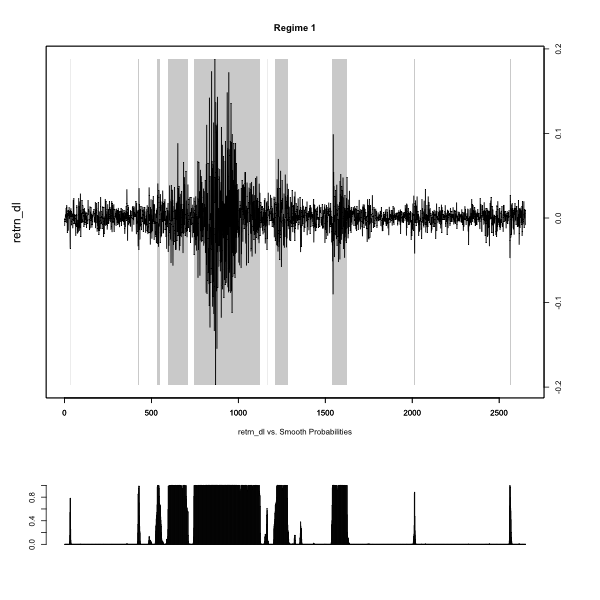
\includegraphics[width=1\textwidth]{../results/regime/RMZ}
\label{fig: RMZregime}
\end{figure}
\end{columns}

\end{frame}

\begin{frame}
\frametitle{Regime switching models--Example: RMZ}
\Fontviii

In order to make a consistent comparison of risk diagnostics between two regimes, we ignore some short discontinuity and pick two longest single occurring episode for each regime. Both episode contain 530 trading days. The episode of regime 1 range from 10/30/2007 to 12/07/2009, and the episode of regime 2 range from 06/20/2013 to 07/29/2015. The right panel shows risk measures of two regimes.

\begin{table}[h]
\centering 
\begin{tabular}{| r | r | r |} 
 \hline
& Regime 1 & Regime 2 \\
& High volatility & Low volatility \\
 \hline 
VaR (empirical, p = 0.95) & 7.4\% & 1.5\% \\
ES (empirical, p = 0.95) & 9.9\% & 2.1\% \\
CED (one-month, p = 0.9) & 38.4\% & 8.4\% \\
Serial correlation (order = 1) & -0.257 & -0.026 \\
Serial correlation (order = 2) & -0.023 & 0.008 \\
 \hline
\end{tabular}
\label{table:ridkDiagsRegimeRMZ}
\caption{Risk diagnostics for RMZ of two equal-length episode of each regime} 
\end{table}

\end{frame}

%------------------------------------------------

\begin{frame}
\frametitle{Regime switching models--Example: RMZ}
\Fontviii

\begin{columns}[c] % The "c" option specifies centered vertical alignment while the "t" option is used for top vertical alignment

\column{.4\textwidth} % Left column and width
The right panel shows the maximum drawdown distributions of two regimes. The regime with high volatility has larger mean, variance, skewness and kurtosis.

\column{.55\textwidth} % Right column and width
\begin{figure}[h]
\centering 
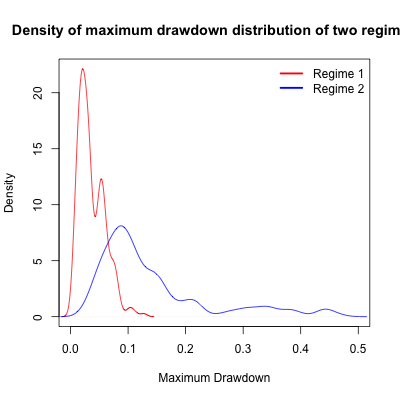
\includegraphics[width=0.8\textwidth]{../results/regime/RMZ_mon1_mdd}
\label{fig: RMZregime_mdd}
\end{figure}
\end{columns}

\end{frame}



%------------------------------------------------
\section{Time Series – GARCH model}
%------------------------------------------------
\subsection{Summary of GARCH Model}
\begin{frame}
\frametitle{Summary of GARCH Model}
\Fontviiii

\begin{table}[!h]
\caption{Best GARCH Model for the residuals after Fitting ARIMA}
\centering 
\begin{tabular}{ | c || r | } 
 \hline
Asset & ARIMA (p,q)+ GARCH(m,n) \\
  \hline \hline
AGG & ARMA(5,5)+GARCH(1,1) \\ 
HYG & ARMA(3,1)+GARCH(1,1) \\ 
TIP &  GARCH(1,1)\\ 
BCOM & GARCH(1,1)\\ 
MXEA & ARMA(2,2)+ GARCH(1,2) \\ 
MXEF & ARMA(4,2) + GARCH(1,1)\\ 
RAY &  ARMA(2,2) + GARCH(1,1)\\ 
RMZ & MA(1) + GARCH(1,1) \\ 
SPX & ARMA(2,2) +GARCH(1,1)\\ 
USGG10YR & GARCH(1,3) \\
 \hline
\end{tabular}
\label{table:BestGarch}
\end{table}
\end{frame}

\subsection{Fit GARCH}
\begin{frame}
\frametitle{RMZ example: Workflow and Diagnostics}
\Fontviii
\begin{columns}[c]
\column{.4\textwidth}
\begin{enumerate}
\item Fit Best ARIMA model, and extract residuals.
\item Select proper GARCH model for the residuals, based on BIC.
\item Check the diagnostic plots
\begin{itemize}
\item Good in general.
\item Heavy Tail.
\end{itemize}
\end{enumerate}
 
 
\column{.6\textwidth} % Right column and width
\begin{figure}[h]
\centering 
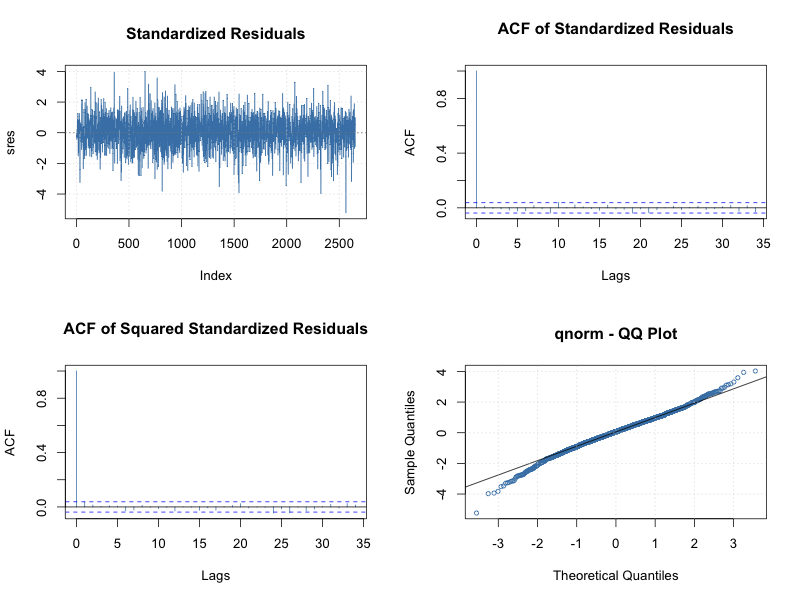
\includegraphics[width=6cm,height = 6cm]{../results/RMZ_GARCH_dig1}
\label{fig:RMZ_GARCH_dig1}
\caption{RMZ example: Diagnostics after Fitting Residual with GARCH(1,1)}
\end{figure}

\end{columns}
\end{frame}

\begin{frame}
\frametitle{RMZ example: Predictions}
\Fontviii
\begin{columns}[c]
\column{.4\textwidth}
\begin{enumerate}
\item Empirical results are similar to the estimation.
\item The second plot give a confident interval for residuals
\item Several steps forward estimation.
\end{enumerate}
 
 
\column{.6\textwidth} % Right column and width
\begin{figure}[h]
\centering 
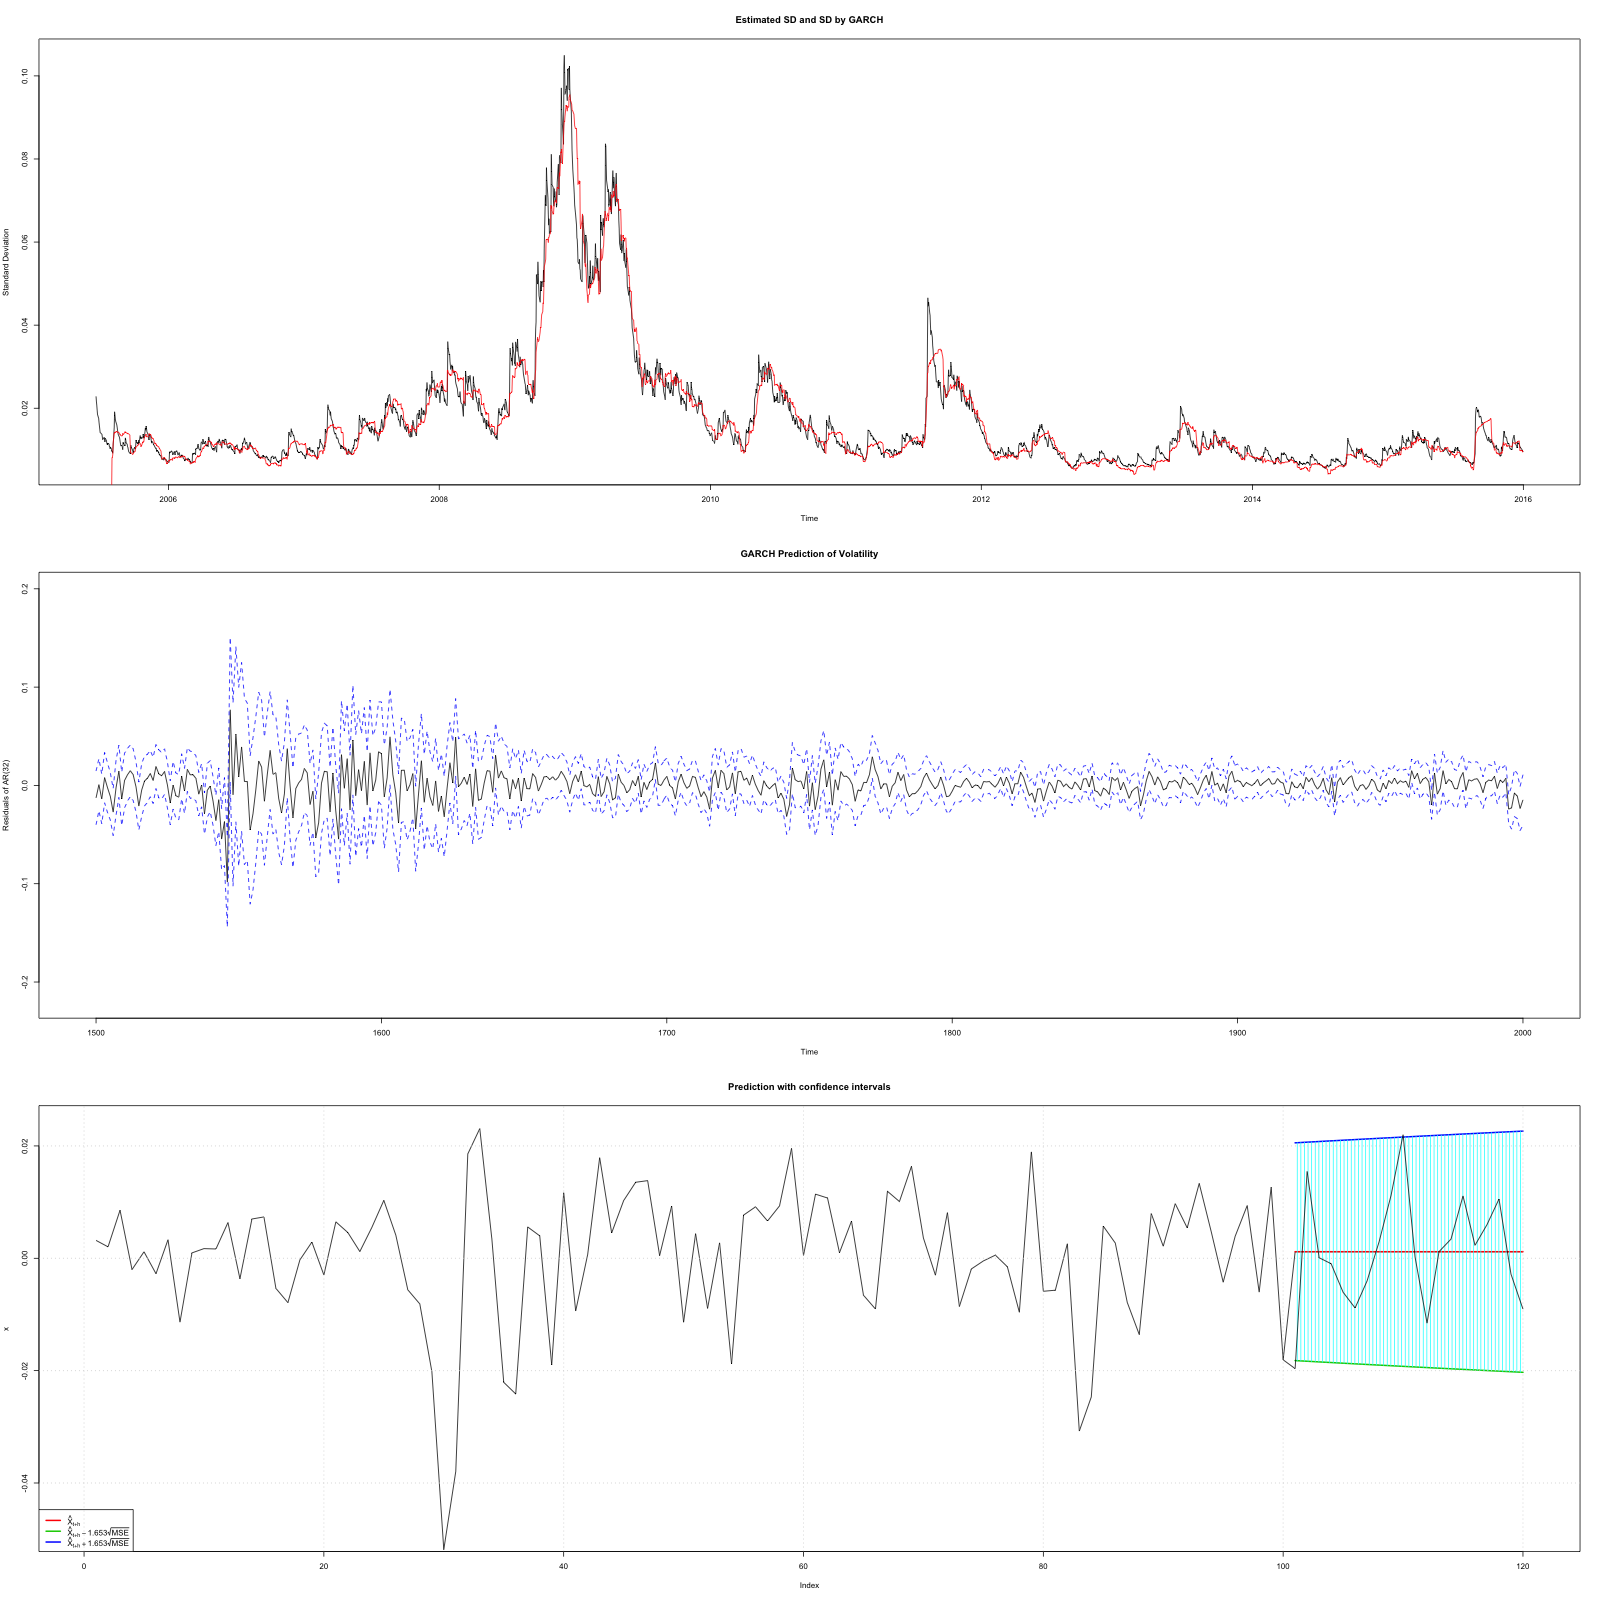
\includegraphics[width=6cm,height = 6cm]{../figures/RMZeg_pred}
\label{fig: dailyReturns}
\caption{RMZ example: Some Prediction Results}
\end{figure}

\end{columns}
\end{frame}

\subsection{Serial Correlation and Risk Measurements}
\begin{frame}
\frametitle{$\kappa(1)$ and CED Using the ``Best" Model}
\Fontviii
\begin{columns}[c]
\column{.4\textwidth}
\begin{enumerate}
\item Almost no pattern there.
\item Correlations are small, and almost negative.
\item Similar to other risk measurement, but less significant
\end{enumerate}
 
 
\column{.6\textwidth} % Right column and width
\begin{figure}[h]
\centering 
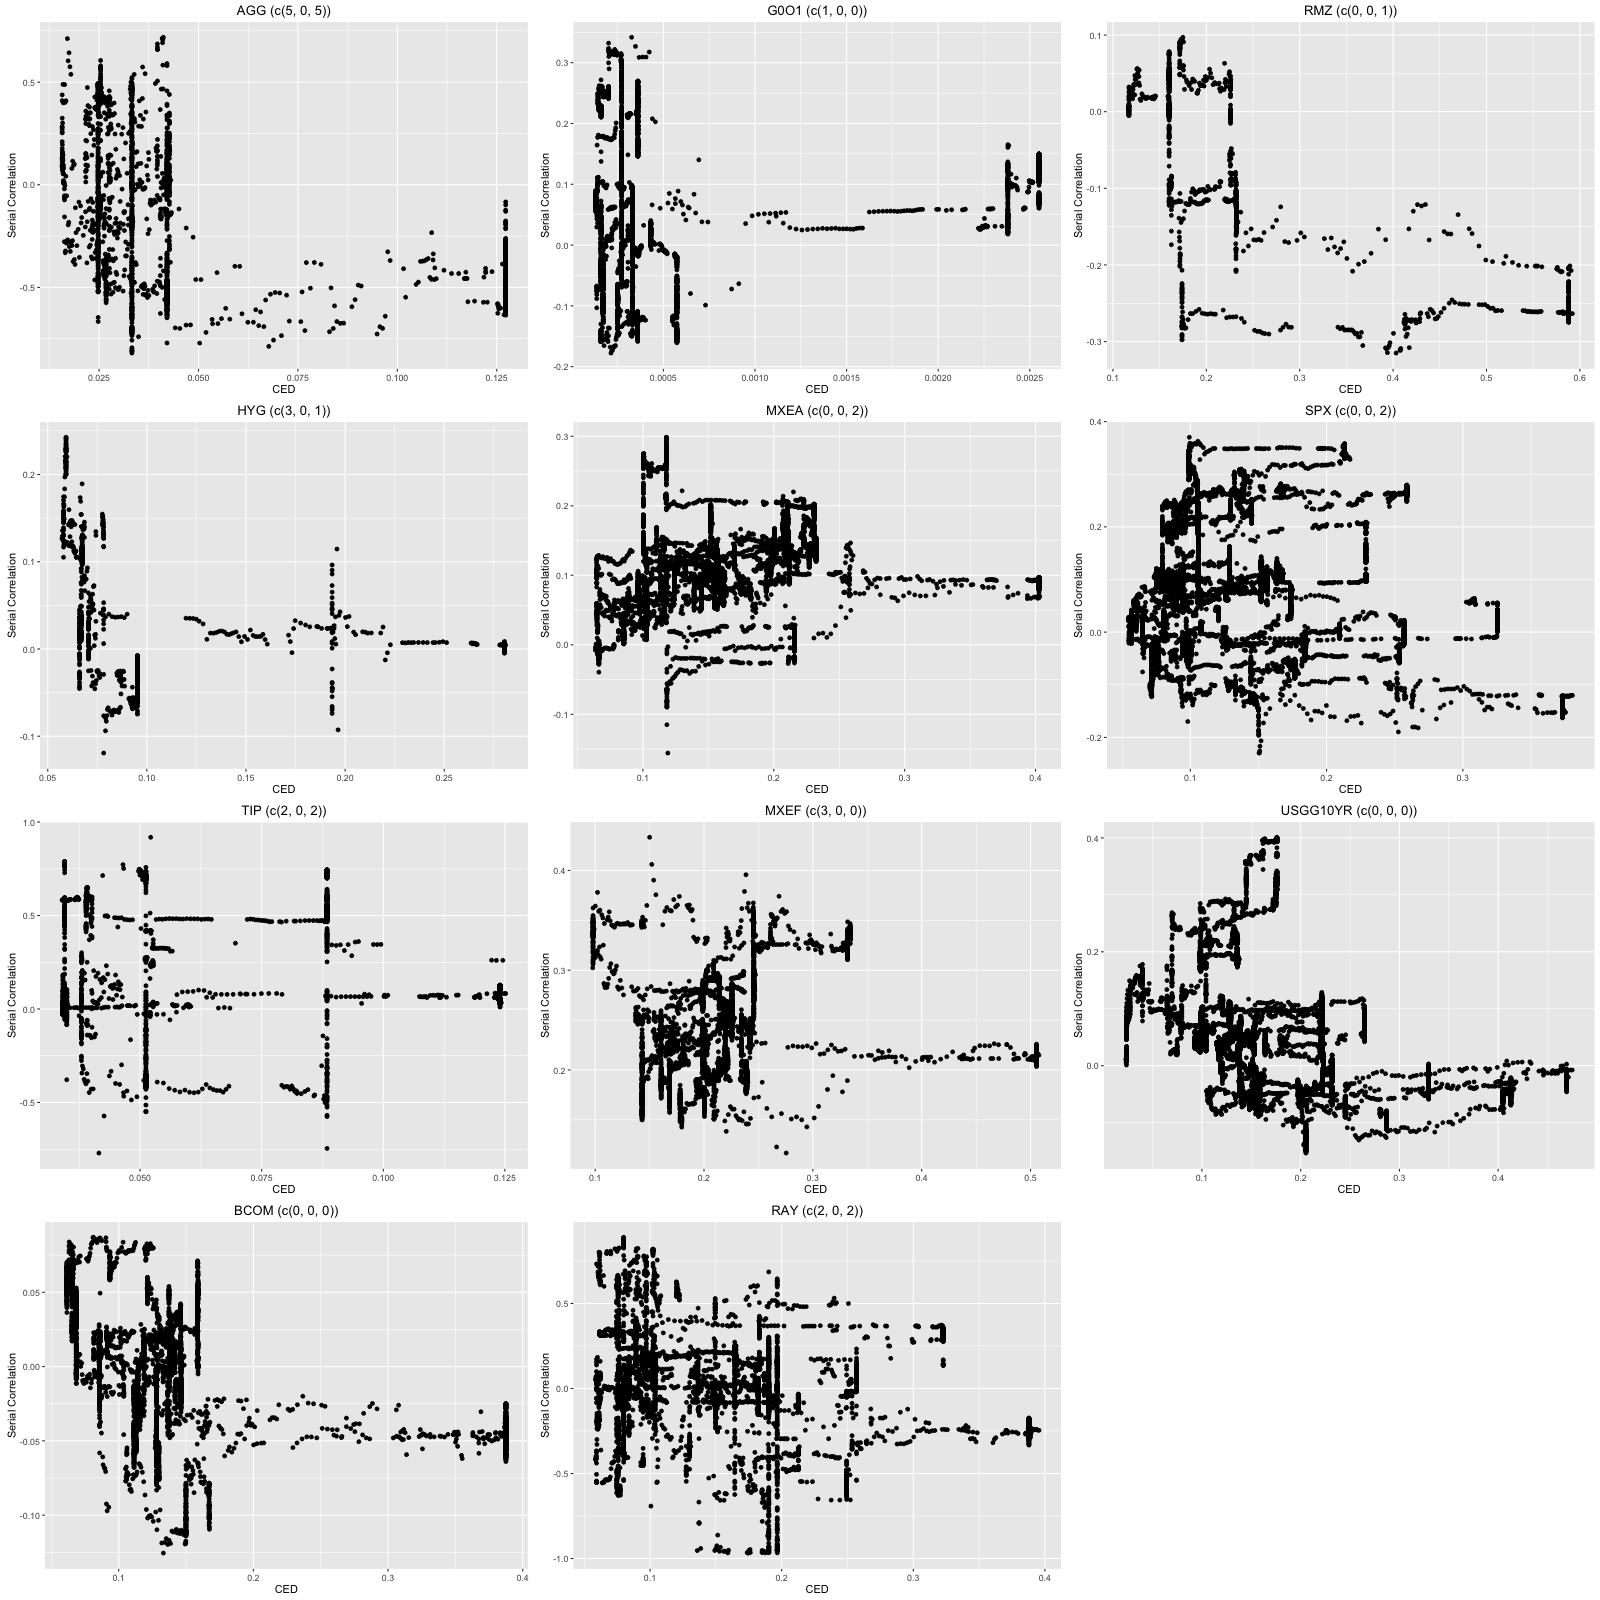
\includegraphics[width=6cm,height = 6cm]{../figures/SerCol-CED3mon2yr}
\label{fig:SerCol-CED3mon2yr}
\caption{$\kappa(1)$ versus CED}
\end{figure}

\end{columns}
\end{frame}

% %------------------------------------------------
% \section{Analysis of weekly and monthly frequencies}
% %------------------------------------------------
% \begin{frame}
% \frametitle{Regime switching models}


% \end{frame}
%------------------------------------------------
\section{Current work: simulation}
%------------------------------------------------
\begin{frame}
\frametitle{Simulation of AR(1) model}
\Fontviii

\begin{figure}[h]
\centering 
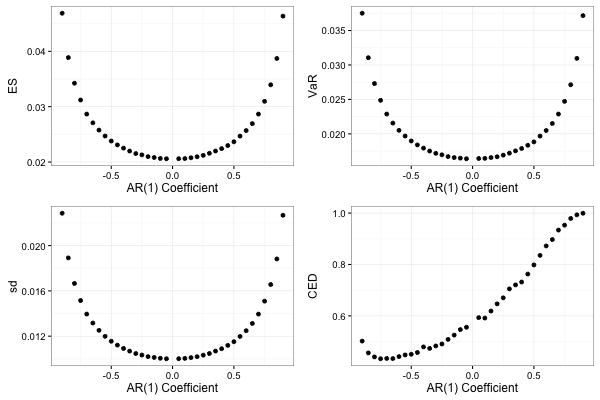
\includegraphics[width=0.7\textwidth]{../figures/AR1_simulation}
\label{fig: CED3mon2yr}
\end{figure}

\end{frame}

%------------------------------------------------

\begin{frame}
\Huge{\centerline{The End}}
\end{frame}

%----------------------------------------------------------------------------------------

\end{document} 